'   \chapter{Referencial Teórico}

Para construir uma análise multivaridade dos casos de câncer de mama em MG, é necessário compreender o contexto e metodologias utilizadas para esta análise multivariada. Sendo assim, é preciso entender 

\section{Conceito de Dados Abertos}
Dados abertos são dados acessíveis ao público, disponibilizados em meio digital, em formato aberto e processável por máquina, referenciados na internet e publicados sob licença que permita uso, reúso e compartilhamento, com a devida atribuição de autoria ou fonte. Além disso, devem ser informados sem barreiras tecnológicas ou jurídicas indevidas que limitem seu aproveitamento social e científico \cite{enap2016dadosabertos}.

\subsection{Princípios de dados governamentais abertos}

Em dezembro de 2007, especialistas em governo aberto reunidos em Sebastopol (Califórnia, EUA) consolidaram oito princípios para orientar políticas de dados governamentais abertos, posteriormente difundidos em iniciativas internacionais de transparência \cite{lopes2023dadosabertos}. Esses princípios são:

\begin{enumerate}
    \item \textbf{Completos:} todos os dados públicos devem ser disponibilizados, respeitando apenas restrições legais legítimas relacionadas a privacidade, segurança e sigilo.

    \item \textbf{Primários:} os dados devem ser publicados em sua forma original, com o maior nível de granularidade possível.

    \item \textbf{Atuais:} a publicação deve ocorrer em tempo adequado para preservar o valor informacional e a utilidade dos dados.

    \item \textbf{Acessíveis:} os dados devem estar disponíveis ao maior número possível de pessoas e para diferentes finalidades de uso.

    \item \textbf{Processáveis por máquina:} os dados devem possuir estrutura que permita leitura e tratamento automatizados.

    \item \textbf{Acesso não discriminatório:} o acesso deve ocorrer sem exigência de cadastro, autenticação restritiva ou tratamento diferenciado de usuários.

    \item \textbf{Formatos não proprietários:} os dados devem ser publicados em formatos abertos, sem dependência de tecnologias de controle exclusivo.

    \item \textbf{Livres de licenças restritivas:} os dados não devem impor limitações indevidas de uso por direitos autorais, patentes ou mecanismos similares, salvo exceções legalmente previstas.
\end{enumerate}



\section{Análise Exploratória de Dados}


As técnicas Exploratory Data Analysis (EDA) são usada para analisar e investigar um conjunto de dados direcionando as principais
características. Determina a melhor forma de controlar as fontes de dados e obter as respostas
necessárias, possibilitando a descoberta de padrões, detecção de anomalias, teste de hipóteses e outras observações. Logo, a importância de utilizar EDA é analisar os dados antes que seja feita
qualquer suposição. Cientistas de dados podem usar a análise exploratória para garantir que os resultados que produzem sejam válidos e aplicáveis a quaisquer objetivos e resultados de negócio desejados. A EDA também ajuda a confirmar se estão sendo feitas as perguntas certas. \cite{ibm2021eda}


\section{Análise Multivariada}
A análise multivariada compreende um conjunto de técnicas estatísticas que analisam simultaneamente múltiplas medidas sobre indivíduos ou objetos sob investigação, de modo que qualquer análise simultânea de mais de duas variáveis pode ser considerada, a princípio, como multivariada \cite{hair2009}. Suas técnicas são extensões da análise univariada e bivariada, ampliando a capacidade analítica ao permitir que relações complexas entre variáveis sejam investigadas em uma única análise, algo que antes exigiria múltiplas análises separadas \cite{hair2009}. Para que seja considerada verdadeiramente multivariada, todas as variáveis devem ser aleatórias e inter-relacionadas de tal forma que seus efeitos não possam ser interpretados de maneira isolada \cite{hair2009}. No contexto deste trabalho, a análise multivariada é aplicada à integração de variáveis epidemiológicas, socioeconômicas e de acesso à saúde dos municípios de Minas Gerais, permitindo identificar padrões e relações que não seriam observáveis por meio de análises individuais de cada variável.

\section{Python e sua popularização na Análise de Dados}

 Desde seu surgimento em 1991, o Python desenvolveu uma comunidade grande e ativa voltada para a computação científica, análise de dados, aprendizado de máquina e desenvolvimento geral de software. \cite{mckinney2022python}


\subsection{Bibliotecas Python}
Existem inúmeras bibliotecas desenvolvidas para a linguagem Python com diversas
aplicações. Nesse tópico é abordado as bibliotecas importantes para o desenvolvimento da
Análise Exploratória realizada nesse projeto.

\subsubsection{Tratamento e Manipulação de Dados}

\paragraph{Pandas} 

\paragraph{NumPy} 

\paragraph{GeoPandas}

\paragraph{geobr} 

\paragraph{openpyxl} 

\subsubsection{Visualização de Dados e Gráficos}

\paragraph{Plotly} 

\paragraph{Matplotlib} 

\subsubsection{Dashboards e Interfaces Interativas}

\paragraph{Dash}

\paragraph{ipywidgets} 

\subsubsection{Web Scraping e Automação}

\paragraph{Selenium} 

\paragraph{webdriver-manager} 

\subsubsection{Gerenciamento de Dependências}

\paragraph{Uv} é um gerenciador de pacotes e projetos Python moderno, escrito em Rust, que oferece performance significativamente superior ao pip/pip-tools. Utilizado neste projeto para definir, resolver e instalar dependências de forma reproduzível através do arquivo \texttt{pyproject.toml}.


\section{Knowledge Discovery in Databases (KDD)}
KDD (Knowledge Discovery in Databases) é o processo não trivial de
identificação de padrões válidos, novos, potencialmente úteis e, finalmente, compreensíveis, em dados. \cite{fayyad1996kdd}. Assim, dados são um conjunto de fatos (por exemplo, casos em um banco de dados), e padrão é uma expressão em alguma linguagem que descreve um subconjunto dos dados ou um modelo aplicável a esse subconjunto. Portanto, extrair um padrão também designa ajustar um modelo aos dados, encontrar estrutura nos dados ou, em geral, fazer qualquer descrição de alto nível de um conjunto de dados \cite{fayyad1996kdd}.

O processo de KDD (Knowledge Discovery in Databases) envolve as seguintes etapas, segundo \cite{han2012datamining}:

\begin{enumerate}
    \item \textbf{Limpeza de dados (Data cleaning):} Para remover ruídos e dados inconsistentes.
    
    \item \textbf{Integração de dados (Data integration):} Onde múltiplas fontes de dados podem ser combinadas.
    \begin{quote}
        \textit{Nota: Uma tendência popular na indústria da informação é realizar a limpeza e a integração como uma etapa de pré-processamento, armazenando os resultados em um Data Warehouse (Armazém de Dados).}
    \end{quote}

    \item \textbf{Seleção de dados (Data selection):} Onde os dados relevantes para a tarefa de análise são recuperados do banco de dados.
    
    \item \textbf{Transformação de dados (Data transformation):} Onde os dados são transformados e consolidados em formas apropriadas para a mineração, através de operações de resumo ou agregação.
    
    \item \textbf{Mineração de dados (Data mining):} Um processo essencial onde métodos inteligentes são aplicados para extrair padrões de dados.
    
    \item \textbf{Avaliação de padrões (Pattern evaluation):} Para identificar os padrões verdadeiramente interessantes que representam conhecimento, baseando-se em medidas de ``interessabilidade'' (grau de utilidade/relevância).
    
    \item \textbf{Apresentação do conhecimento (Knowledge presentation):} Onde técnicas de visualização e representação de conhecimento são usadas para apresentar o conhecimento minerado aos usuários.
\end{enumerate}

A Figura a seguir ilustra a sequência lógica desse processo, que abrange desde a requisição inicial até a estruturação final dos dados.


\begin{figure}[!htb]
    \centering
    \begin{minipage}{0.7\textwidth}
        \caption{Arquitetura de funcionamento de um Web Scraper}
        \label{fig:KDD}
        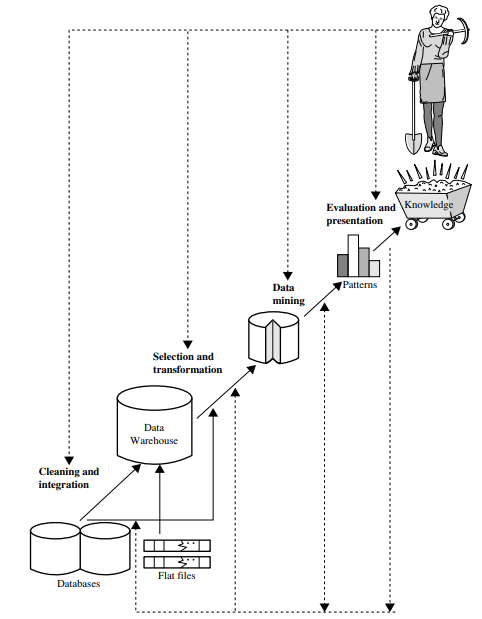
\includegraphics[width=\textwidth]{Imagens/KDD.png}
        \caption*{\footnotesize Fonte: \textcite{anuradha2015brief}.}
    \end{minipage}
\end{figure}

\section{Web Scraping}

O web scraping, também conhecido como raspagem de dados da web, refere-se ao processo automatizado de extração de informações de páginas da Internet. Esse processo envolve a utilização de programas (\textit{scrapers} ou \textit{crawlers}) capazes de navegar por websites, identificar conteúdos específicos e transformá-los em formato estruturado para posterior análise \cite{glez2013scraping}.

De acordo com \textcite{mitchell2018scraping}, o funcionamento básico de um \textit{web scraper} pode ser descrito nas seguintes etapas:

\begin{enumerate}
    \item \textbf{Requisição:} envio de solicitações HTTP para os endereços de interesse, simulando o comportamento de um navegador.
    \item \textbf{Carregamento e análise:} leitura do HTML retornado e identificação dos elementos relevantes.
    \item \textbf{Extração:} coleta dos dados por meio de regras definidas, como seletores CSS, XPath ou expressões regulares.
    \item \textbf{Estruturação:} organização dos dados em formatos como CSV, JSON ou tabelas em banco de dados.
    \item \textbf{Armazenamento:} persistência das informações para consulta e análises posteriores.
\end{enumerate}

Uma arquitetura típica de web scraping envolve, inicialmente, a definição de palavras-chave em um mecanismo de busca para obtenção de URLs relevantes. Em seguida, um componente de \textit{crawling} visita essas páginas e coleta seu conteúdo, que é processado pelo \textit{scraper} e convertido em arquivos estruturados para uso analítico \cite{anuradha2015brief}.

\begin{figure}[!htb]
    \centering
    \begin{minipage}{0.8\textwidth}
        \caption{Arquitetura de funcionamento de um Web Scraper}
        \label{fig:webScraperIngles}
        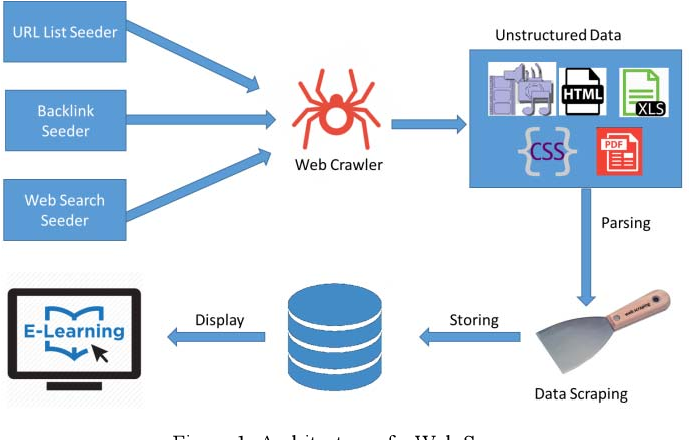
\includegraphics[width=\textwidth]{Imagens/webScraperIngles.png}
        \caption*{\footnotesize Fonte: \textcite{anuradha2015brief}.}
    \end{minipage}
\end{figure}



% A web está repleta de textos, muitos dos quais organizados em tabelas, alimentados por bancos de dados ou incorporados em arquivos PDF. A maior parte dessas informações, contudo, é estruturada por meio de tags de marcação HTML ou XHTML, que orientam os navegadores sobre como exibi-las ao usuário. 

% Nesse contexto, Web Scraping surge como uma técnica para a automação da coleta de informações em ambientes digitais, possibilitando a extração de dados estruturados e não estruturados disponíveis em páginas da web \cite{abodayeh2023scraping}. 




% O web scraping, também conhecido como web crawling ou raspagem de dados da
% web, refere-se ao processo automatizado de extração de informações de páginas da Internet. Esse processo envolve a utilização de web scrapers, conhecidos como scrapers ou crawlers, que navegam pelos websites, identiĄcam e capturam dados especíĄcos, transformandoos em um formato estruturado para posterior análise, conforme pode ser observado na
% Figura 1. Os web scrapers podem ser projetados para coletar textos, imagens, tabelas e
% outros elementos presentes nas páginas web (GLEZ-PEijA et al., 2013). \cite{glez2013scraping
% }

% De acordo com Mitchell (2018) \cite{mitchell2018scraping} funcionamento básico de um web scraper envolve os seguintes passos:

% Requisição: O web scraper envia solicitações HTTP para links específicos, simulando o comportamento de um navegador;

% Carregamento e Análise: O HTML da página web é carregado e analisado pelo web scraper para identificar os elementos relevantes a serem extraídos;

% Extração: Os dados desejados são extraídos do HTML, seguindo padrões definidos, como seletores CSS ou expressões regulares;

% Estruturação: Os dados extraídos são transformados em um formato estruturado, como CSV, JSON ou bancos de dados;

% Armazenamento: Os dados estruturados podem ser armazenados localmente ou em sistemas de gerenciamento de dados. 
% presenta-se na Figura 2 uma arquitetura de um Web scraper no qual as palavraschave são executadas em um mecanismo de pesquisa e, com base nas configurações de
% parâmetros, são produzidos cerca de oito a dez links da Web por palavra-chave. Os links
% são então enviados para o “Semeador de listas de URL”, que usa um Web crawler para
% extrair o conteúdo dos sites visitados. O conteúdo coletado é então passado para um
% scraper e enviado na forma de arquivos de texto para uma estação de trabalho
% (UPADHYAY et al., 2017).
% \lipsum[1] \ref{fig:webScraperIngles} \cite{anuradha2015brief}


% Aplicações tecnológicas com grande capacidade de coleta de dados como o Web Scraping é uma forma de mineração de dados e o objetivo geral do processo de scraping é coletar dados e informações de sites e transformá-las em uma estrutura compreensível, como planilhas, banco de dados ou um arquivo Comma Separated Values (CSV) ou valores separados por vírgula \cite{dastidar2016pir}


% \lipsum[1] \ref{fig:Stack} \cite{anuradha2015brief}

% \begin{figure}[!htb]
%     \centering
%     \begin{minipage}{0.8\textwidth}
%         \caption{\label{fig:Stack} Pilha de Tecnologias utilizadas em Big Data}
%         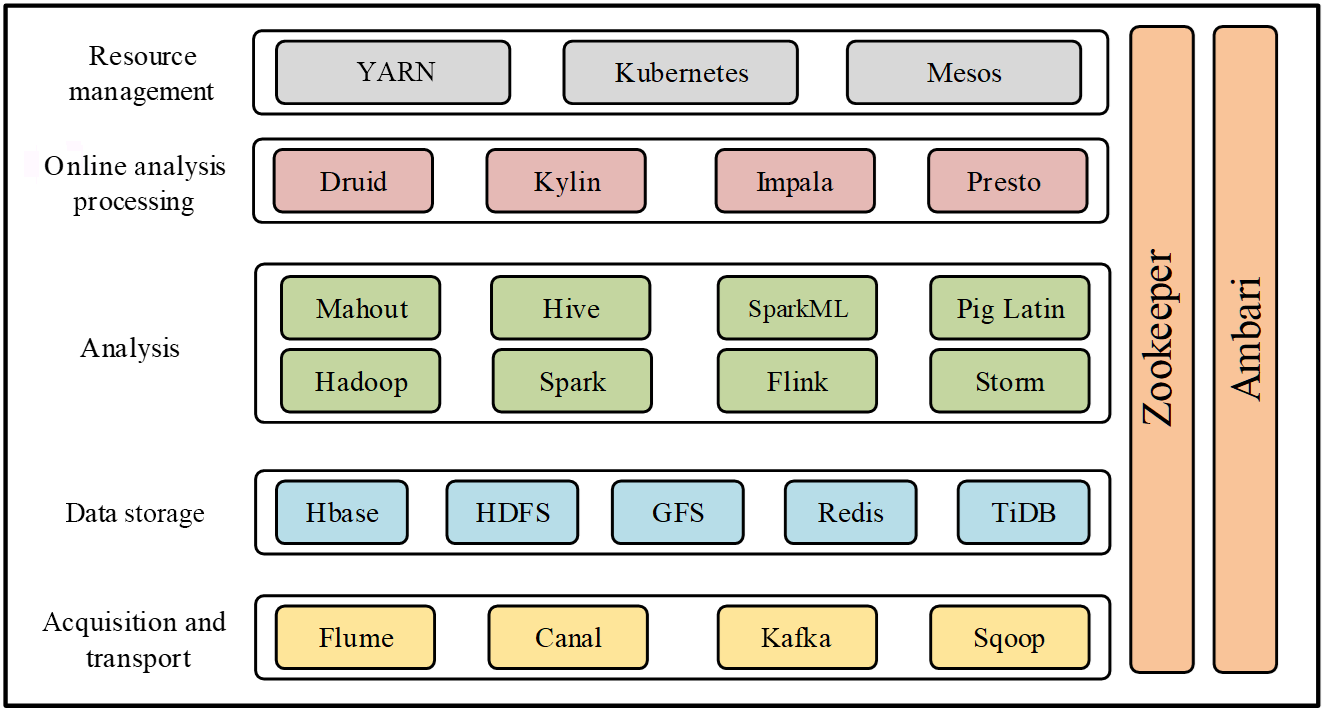
\includegraphics[width=\textwidth]{Imagens/Stack.png}
%         \caption*{\footnotesize Fonte: \textcite{sun2023survey}.}
%     \end{minipage}
% \end{figure}

% \lipsum[6]

% \section{Seção}
% \lipsum[2]
% \cite{anuradha2015brief}
% \subsection{SubSeção}
% \lipsum[3]
% \cite{anuradha2015brief}
% \subsubsection{SubSubSeção}
% \lipsum[4]

